\documentclass{mwart}
\usepackage{multicol}
\usepackage{polski} % Pozwala na użycie polskiego. Ustawia między innymi fontenc na T1
\usepackage[utf8]{inputenc} % Informuje o kodowaniu
\usepackage{enumitem}
\usepackage{xcolor}
\usepackage{xcolor}% http://ctan.org/pkg/xcolor
\usepackage{hyperref}
\usepackage{listings}
\usepackage{float} % Ustawianie obrazów
\usepackage[caption = false]{subfig} % Wiele obrazów w jednej figurze
\definecolor{LinkColor}{HTML}{1d5cc1}
\renewcommand{\labelitemi}{\textbullet} % Zmiana symbolu wliczeń

\lstset{
  basicstyle=\ttfamily,
  columns=fullflexible,
  breaklines=true,
  postbreak=\mbox{\textcolor{red}{$\hookrightarrow$}\space},
}

\definecolor{LinkColor}{HTML}{1d5cc1}

\usepackage{tabto}

\usepackage{graphicx} % Pakiet do obrazów
\graphicspath{ {./Obrazy/} } % Folder, z którego będą brane obrazy

% Nie twórz nowych stron
\usepackage{etoolbox}
\makeatletter
% \patchcmd{\chapter}{\if@openright\cleardoublepage\else\clearpage\fi}{}{}{}
\makeatother

\newcommand{\paragraphnl}[1]{\paragraph{#1} \mbox{} \\} % Paragraf z nową linią

\title{PRIR Specyfikacja wstępna - Gra w życie}
\author{Krzysztof Dąbrowski 293101}
\date{\today}

\begin{document}
\maketitle{}

\tableofcontents{}

\section{Opis zadania}
Projekt polega na zrealizowaniu równoległej symulacji \textit{Gry w życie}.
W tym celu zostanie rozbudowany projekt z przedmiotu JIMP2. 
W przeciwieństwie do większości zadań realizowanych na uczelni, w ramach projektu zostanie rozbudowany już istniejący kod.
Zadanie to będzie wymagało innego podejścia, co moim zdaniem dobrze pasuje do aspektów programowania równoległego, które pozwala na przyśpieszenie już istniejących rozwiązań.

Projekt zakłada przygotowanie równoległej symulacji w językach Java oraz C.
Dzięki temu możliwe będzie porównanie użytych bibliotek, architektur kodu oraz wydajności otrzymanych rozwiązań.

\section{Opis ogólny problemu}
Gra w życie jest automatem komórkowym wymyślonym przez brytyjskiego matematyka John Horton Conway
w 1970 roku. Polega na symulacji kolejnych pokoleń życia komórek według następujących zasad.

\subsection{Symulacja}

\paragraph{Stany} Komórka może znajdować się w jednym z dwóch stanów:
\begin{itemize}
\item żywa,
\item martwa.
\end{itemize}

\paragraph{Pokolenie} to stan wszystkich komórek w danej chwili. Gdy stan pokolenia jest ustalony, możliwe jest utworzenie nowego (potomnego) pokolenia komórek, powstających według poniższych zasad.

\paragraph{Reguły} Następne pokolenie generowane jest zgodnie z regułami:
\begin{itemize}
\item Jeżeli komórka była martwa i miała dokładnie 3 żywych sąsiadów, w następnym pokoleniu staje się żywa,
\item Jeżeli komórka była żywa to pozostaje żywa jeśli miała dwóch lub trzech żywych sąsiadów. W przeciwnym razie staje się martwa.
\end{itemize}

\subsection{Struktury}
Symulacja przeprowadzona zgodnie z powyższymi regułami może prowadzić do powstania ciekawych obiektów zwanych strukturami. 

\begin{figure}[h]
\centering
\setlength{\fboxsep}{0pt} %Odstęp 0
\setlength{\fboxrule}{1pt} %Grubość ramki 1p
\fbox{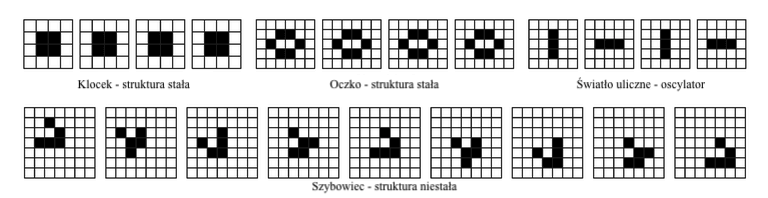
\includegraphics[width=13cm]{struktury}}
\caption{Przykłady struktur}
\end{figure}

Reguły symulacji umożliwiają również tworzenie dużo bardziej skomplikowanych struktur (jak na przykład maszyna Turinga -- https://youtu.be/My8AsV7bA94).

\section{Opis funkcjonalności}
Ponieważ rozbudowywane są dwa różne programy to funkcjonalności będą zależne od programu.

\subsection{Rozwiązanie w języku Java}
Program wyświetla interface graficzny pozwalający na wykonywanie symulacji automatów komórkowych \textit{Gra w życie} oraz \textit{Wireworld}.
Użytkownik może wygenerować losowy automat komórkowy lub stworzyć własny przy pomocy narzędzi pozwalających na modyfikację stanu wybranych komórek.
Możliwa jest automatyczna symulacja lub ręczne przechodzenie między kolejnymi stanami.
Dany stan automatu może zostać zapisany do pliku oraz później wczytany.

\subsection{Rozwiązanie w języku C}
Program działa w trybie wsadowym.
Użytkownik przy pomocy argumentów wiersza poleceń może ustalić opisane poniżej parametry symulacji.

\paragraph{Argumenty} \label{argumenty}
\begin{itemize}
\item \texttt{-h / --help} \\ Wyświetlenie pomocy,
\item \texttt{ -f [nazwa pliku]  / --file plik [nazwa pliku] } 
	\\ \textit{ Łańcuch znaków }będący nazwą pliku z wejściowym stanem planszy zgodny z \hyperref[format]{\textcolor{LinkColor}{formatem}}; wyklucza się z  \hyperref[s]{\textcolor{LinkColor}{flagą -s}}
\item \texttt{-o [ścieżka] / --output\textunderscore{}dest [ścieżka]}  \\\textit{ Łańcuch znaków }będący ścieżką do folderu, w którym zostaną zapisane wyniki \label{output_dest} symulacji. Domyślnie pliki  będą generowane w folderze  o nazwie będącej aktualną datą i godziną wywołania programu,
\item \texttt{-t [gif | png | txt] / --type [gif | png | txt])} \\\textit{ Łańcuch znaków }reprezentujący typ generowanych rezultatów. Domyślnie gif, \label{output_args}
\item \texttt{-n [liczba] / --number\textunderscore{}of\textunderscore{}generations [liczba]} \\ \textit{ Liczba } pokoleń do wygenerowania. Domyślnie 15,
\item \texttt{-p [liczba] / --step [liczba]} \\ \textit{ Liczba }decydująca o tym, co który stan symulacji będzie zapisywany. Domyślnie 1,
\item \label{s} \texttt{-s [LICZBAxLICZBA] / --size [LICZBAxLICZBA]} \\ \textit{ Łańcuch znaków } o formacie "XxY" (X -- szerokość planszy, Y -- wysokość planszy), będący wymiarami losowo generowanej planszy początkowej. Wyklucza się z -f, 
\item \label{delay} \texttt{-d [liczba] / --delay [liczba]} \\ Podanie tego argumentu spowoduje wyświetlanie w konsoli kolejnych pokolenie symulacji. \textit{ Liczba } ta będzie oznaczać czas  w milisekundach między wyświetleniem poszczególnych pokoleń. Wartość -1, co oznacza manualne przechodzenie do następnego pokolenia klawiszem ENTER lub zapisanie wyświetlanego pokolenia w pliku.txt wpisując ,,save''.
\end{itemize}

Wywołanie programu bez żadnego argumentu przyjmuje flagę --size 10, i wartości domyślne innych parametrów.

Wyniki symulacji są wyświetlana na konsolę lub zapisywane do plików o wybranym formacie.

\section{Analiza możliwości zrównoleglenia programu}
Liczenie stanu każdej komórki w danym pokoleniu zależy tylko od stanu komórek sąsiednich w poprzednim pokoleniu. Dzięki temu możliwe jest niezależne symulowanie każdej komórki nowego pokolenia.
Nie da się jednak symulować przyszłych pokoleń nie znając stanu pokolenia poprzedniego.

Do symulacji tak zadanego problemu bardzo dobrze nadaje się zastosowanie wątków oraz pamięci współdzielonej.

Teoretyczne przyśpieszenie jakie można uzyskać poprzez zrównoleglenie programu jest równe liczbie zastosowanych wątków.

\section{Wybór technologii}
Do zrównoleglenia aplikacji w języku Java zastosowane będzie współczesne \textit{Stream API} z wykorzystaniem \textit{parallel stream}. Ponieważ na wcześniejsze zadania laboratoryjne wykorzystywałem klasy \texttt{Tread} to takie podejście pozwoli na zaznajomienie się z innym sposobem zrównoleglania obliczeń w tym języku.

Do projektu w C zastosowane będą \textit{posix thread} lub ewentualnie \textit{OpenMP}.
Z uwagi na potencjalną trudność dodania \textit{OpenMP} do już istniejącego projektu bardziej prawdopodobne jest zastosowanie wątków.

\section{Opis sposobu zrównoleglenia}
Ponieważ stan kolejnego pokolenia bazuje na pokoleniu poprzednim możliwe jest tylko zrównoleglenie symulacji jednego pokolenia w przód.

Zrównoleglenie symulacji danego pokolenia może być wykonane na dwa sposoby.
Można wykonać zrównoleglenie wykonania poprzez podział całej planszy na obszary, które będą oddzielnie symulowane przez poszczególne wątki.
Alternatywnie możliwe jest obliczanie przez wątki kolejnych pól po kolei przy pomocy schematu \textit{round-robin}.

Zastosowanie przydziału \textit{round-robin} pozwoli na zminimalizowanie oczekiwania na najwolniejszy wątek, może jednak powodować narzuty związane z pobieraniem kolejnych danych przez wątki.
Optymalnym podejściem może być połączenie obu metod, polegające na cyklicznym przetwarzaniu bloków po kila komórek przez poszczególne wątki.

\end{document}
